\documentclass[11pt,fleqn]{article} 
\usepackage[margin=0.8in, head=0.8in]{geometry} 
\usepackage{amsmath, amssymb, amsthm}
\usepackage{fancyhdr} 
\usepackage{palatino, url, multicol}
\usepackage{graphicx, pgfplots} 
\usepackage[all]{xy}
\usepackage{polynom,tabularx} 
%\usepackage{pdfsync} %% I don't know why this messes up tabular column widths
\usepackage{enumerate}
\usepackage{framed}
\usepackage{setspace}
\usepackage{array}
\usepackage{pgf,tikz}
\usepackage{mathrsfs}

\usepackage[parfill]{parskip}
\usetikzlibrary{arrows}

\usetikzlibrary{calc}

\pgfplotsset{compat=1.6}

\pgfplotsset{soldot/.style={color=blue,only marks,mark=*}} \pgfplotsset{holdot/.style={color=blue,fill=white,only marks,mark=*}}

\renewcommand{\headrulewidth}{0pt}
\newcommand{\blank}[1]{\rule{#1}{0.75pt}}
\newcommand{\bc}{\begin{center}}
\newcommand{\ec}{\end{center}}
\newcommand{\be}{\begin{enumerate}}
\newcommand{\ee}{\end{enumerate}}

\renewcommand{\d}{\displaystyle}

\newcommand{\ans}[1][2]{ \ \rule{#1 in}{.5 pt} \ }


\pagestyle{fancy} 
%\lfoot{Uses a calculator}
\rfoot{4-7 (day 1)}

\begin{document}

\vspace*{-0.7in}

\begin{center}
  \Large\sc{Section 4.7 Optimization (Day 1)}\\
\end{center}
\begin{enumerate}
\item A Framework for Approaching Optimization
\begin{enumerate}
\item Identify the quantity to be minimized or maximized.
\item Chose notation and explain what it means.
\item Write the thing you want to maximize or minimize \textbf{as a function of one variable}, including a reasonable \textbf{domain}.
\item Use calculus to answer the question and \emph{justify} that your answer is correct.
\end{enumerate}
Read the problem two or three times. Draw pictures. Label them. Pick specific numerical examples, to make the problem concrete. Be creative. Try more than just one approach. Organization matters.
\item  Find two positive numbers whose sum is 110 and whose product is a maximum.
\vfill
\newpage
\item A rancher has 800 feet of fencing with which to
  enclose three adjacent rectangular corrals. See figure below. What dimensions should
  be used so that the enclosed area will be a maximum?\\
  
  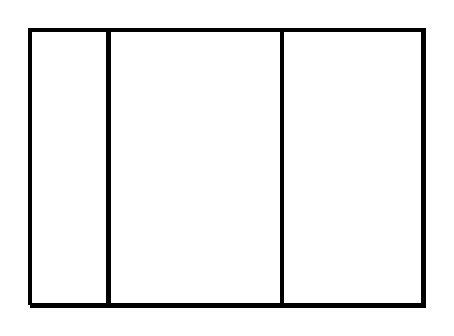
\begin{tikzpicture}
  \draw[ultra thick] (0,0) -- (5,0) -- (5,3.5) -- (0,3.5) -- (0,0);
  \draw[ultra thick] (1,0)--(1,3.5) (3.2,0)--(3.2,3.5);
  \end{tikzpicture}
\vfill
\item Which points on the graph of $y = 4-x^2$ are
  closest to the point $(0, 2)$? (Get started on this problem and once you have a function -- that is, you have made it through part (d) of the Framework -- look at the hint at the bottom of the page.)
  \vfill
  HINT: Whenever you are asked to maximize or minimize distance, it is nearly ALWAYS easier to maximize or minimize the \emph{square} of the distance. Why? 
\end{enumerate}
\end{document}
